% Created 2025-06-08 Sun 08:16
% Intended LaTeX compiler: pdflatex
\documentclass[aspectratio=169]{beamer}
\usepackage[utf8]{inputenc}
\usepackage[T1]{fontenc}
\usepackage{graphicx}
\usepackage{longtable}
\usepackage{wrapfig}
\usepackage{rotating}
\usepackage[normalem]{ulem}
\usepackage{amsmath}
\usepackage{amssymb}
\usepackage{capt-of}
\usepackage{hyperref}
\usepackage[style=apa, backend=biber]{biblatex}
\DeclareLanguageMapping{american}{american-apa}
\addbibresource{./refs/refs.bib}
\AtEveryBibitem{\clearfield{note}}
\usepackage{endnotes}
\let\footnote=\endnote
\usepackage{./jtc}
\usetheme{default}
\author{Evan Misshula}
\date{\today}
\title{Introduction to Machine Learning Modeling, Training and Evaluation}
\hypersetup{
 pdfauthor={Evan Misshula},
 pdftitle={Introduction to Machine Learning Modeling, Training and Evaluation},
 pdfkeywords={},
 pdfsubject={},
 pdfcreator={Emacs 29.3 (Org mode 9.6.15)}, 
 pdflang={English}}
\begin{document}

\maketitle
g
\section{Workflow}
\label{sec:orgc917d96}
\begin{frame}[label={sec:org2f77b01}]{End to end process}
Recall \alert{ML workflow} is a sequence of steps to build and deploy a model that
solves a problem using data.
\end{frame}

\begin{frame}[label={sec:org0e60057}]{The pipeline}
:BEAMER\textsubscript{env}: block
:END:

\begin{center}
\begin{tabular}{llll}
Ingestion \& Preprocessing & Analysis & \alert{Modeling} & Deployment\\[0pt]
\hline
Definition & EDA & \alert{Selection} & Tuning\\[0pt]
Data Collection & Feature Engineering & \alert{Training} & Deployment\\[0pt]
Cleaning &  & \alert{Evaluation} & Monitoring\\[0pt]
\end{tabular}
\end{center}
\end{frame}

\begin{frame}[label={sec:org62e5be9}]{ML Workflow Graph}
\begin{figure}[htbp]
\centering
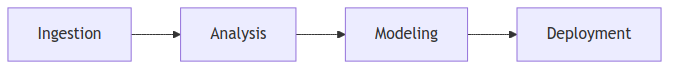
\includegraphics[width=.9\linewidth]{workflow.png}
\caption{ML workflow steps rendered as a flowchart}
\end{figure}


\begin{center}
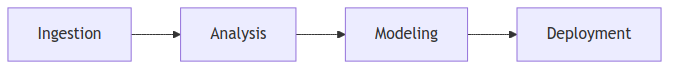
\includegraphics[width=.9\linewidth]{workflow.png}
\end{center}
\end{frame}

\section{Training}
\label{sec:org8a5192f}
\begin{frame}[label={sec:org2f736fd}]{What is Model Training?}
\begin{itemize}
\item Model training is the process of estimating parameters \(\theta\) of a model \(f_\theta(x)\) using data \(\{(x_i, y_i)\}_{i=1}^n\).
\item Typically achieved by minimizing a loss function:
\begin{equation}
\hat{\theta} = \arg\min_\theta \frac{1}{n} \sum_{i=1}^n \mathcal{L}(f_\theta(x_i), y_i)
\end{equation}
\item Common loss functions:
\begin{itemize}
\item \alert{\alert{Squared error loss}} (regression): \(\mathcal{L}(\hat{y}, y) = (\hat{y} - y)^2\)
\item \alert{\alert{Cross-entropy loss}} (classification):
\end{itemize}
\end{itemize}
\begin{equation}
    \mathcal{L}(\hat{y}, y) = -\sum_{c} \1_{\{y = c\}} \log \hat{p}_c
\1_{\{x = 1\}}
\end{equation}
\end{frame}



\begin{frame}[label={sec:org4a97d31}]{Training vs Generalization}
\begin{itemize}
\item \alert{\alert{Empirical risk}} (training error):
\begin{equation}
\hat{R}(\theta) = \frac{1}{n} \sum_{i=1}^n \mathcal{L}(f_\theta(x_i), y_i)
\end{equation}
\item \alert{\alert{Expected risk}} (true/generalization error):
\begin{equation}
R(\theta) = \mathbb{E}_{(x,y) \sim \mathcal{D}} \left[ \mathcal{L}(f_\theta(x), y) \right]
\end{equation}
\item Generalization gap: \(R(\theta) - \hat{R}(\theta)\)
\item Overfitting: small \(\hat{R}\), large \(R\)
\end{itemize}
\end{frame}

\section{Evaluation}
\label{sec:org2060ddc}
\begin{frame}[label={sec:orgd7f121d}]{Evaluation Metrics}
\begin{itemize}
\item \alert{Regression}:
\begin{itemize}
\item Mean Squared Error (MSE): 
\[
    \text{MSE} = \frac{1}{n} \sum_{i=1}^n (\hat{y}_i - y_i)^2
    \]
\item \(R^2\) score:
\[
    R^2 = 1 - \frac{\sum_i (\hat{y}_i - y_i)^2}{\sum_i (y_i - \bar{y})^2}
    \]
\end{itemize}

\item \alert{Classification}:
\begin{itemize}
\item Accuracy: \(\text{Accuracy} = \frac{1}{n} \sum_{i=1}^n \mathds{1}_{\{\hat{y}_i = y_i\}}\)
\item Precision: \(\frac{\text{TP}}{\text{TP} + \text{FP}}\)
\item Recall: \(\frac{\text{TP}}{\text{TP} + \text{FN}}\)
\item F1 score: harmonic mean of precision and recall
\[
    F1 = 2 \cdot \frac{\text{Precision} \cdot \text{Recall}}{\text{Precision} + \text{Recall}}
    \]
\end{itemize}
\end{itemize}
\end{frame}

\begin{frame}[label={sec:orgcaca220}]{Cross-Validation}
\begin{itemize}
\item Cross-validation estimates generalization error by partitioning data.
\item \alert{k-fold CV}:
\begin{itemize}
\item Split data into \(k\) disjoint subsets.
\item For each \(i = 1, \ldots, k\):
\begin{itemize}
\item Train on \(k-1\) folds
\item Evaluate on fold \(i\)
\end{itemize}
\item Average the evaluation metrics.
\end{itemize}
\end{itemize}
\end{frame}

\begin{frame}[label={sec:org2c6b2ca}]{Bias-Variance Tradeoff}
\begin{itemize}
\item Expected prediction error at point \(x\):
\[
  \mathbb{E}[(f(x) - y)^2] = \underbrace{[\mathbb{E}(f(x)) - y]^2}_{\text{Bias}^2} + \underbrace{\mathbb{E}[(f(x) - \mathbb{E}(f(x)))^2]}_{\text{Variance}} + \underbrace{\sigma^2}_{\text{Irreducible error}}
  \]
\item Simple models: low variance, high bias
\item Complex models: low bias, high variance
\end{itemize}
\end{frame}

\begin{frame}[label={sec:org33c1634}]{Model Selection}
\begin{itemize}
\item Choose the best model using a \alert{validation set} or \alert{cross-validation}.
\item Avoid tuning hyperparameters using the test set.
\item Balance:
\begin{itemize}
\item Training error
\item Generalization performance
\item Computational cost
\end{itemize}
\end{itemize}
\end{frame}

\begin{frame}[label={sec:orgf655c04}]{Summary Training and Evaluation}
\begin{itemize}
\item Training minimizes empirical loss.
\item Evaluation uses test or validation data.
\item Use metrics appropriate for the task.
\item Cross-validation provides robust error estimates.
\item The bias-variance tradeoff is fundamental in choosing models.
\end{itemize}
\end{frame}
\end{document}
